\documentclass[11pt,a4paper]{article}

\usepackage[margin=2.3cm]{geometry}
\usepackage{amsmath,amssymb,amsthm,bm}
\usepackage{graphicx}
\usepackage{booktabs}
\usepackage{siunitx}
\usepackage[numbers,sort&compress]{natbib}
\usepackage{caption}
\usepackage{subcaption}
\usepackage[section]{placeins}
\usepackage{tikz}
\usetikzlibrary{arrows.meta,positioning,fit}
\usepackage[hidelinks]{hyperref}

\graphicspath{{figures/}}
\sisetup{per-mode=symbol}
\captionsetup{font=small,labelfont=bf}
\newtheorem{proposition}{Proposition}
\newcommand{\pd}[2]{\frac{\partial #1}{\partial #2}}
\newcommand{\PMtwo}{PM$_{2.5}$}

\title{Physics-Informed Neural Networks for Urban Air Pollution Modelling:\\
Analysis, Simulation and Prediction of \PMtwo{} over Delhi}
\author{Mathematical Modelling Group Project\\[2pt]
\small Member 1 \quad Member 2 \quad Member 3 \quad Member 4 \quad Member 5}
\date{November 2026}

\begin{document}
\maketitle

\begin{abstract}
We model the hourly, mixing-layer-averaged concentration of fine particulate matter (\PMtwo) over Delhi
with a two-dimensional, time-dependent advection--diffusion--reaction (ADR) equation and embed it in a
physics-informed neural network (PINN). Wind and boundary-layer height are taken from the ERA5
reanalysis; the eddy diffusivity, a spatial emission field and a diurnal emission profile are learned.
We analyse the equation (non-dimensionalisation, Fourier stability and equilibrium, mass balance,
positivity, identifiability and forward sensitivity), verify our implementation against an exact Gaussian-puff
solution, and evaluate the PINN in two settings, always on monitoring stations withheld from training:
(i) a synthetic twin in which the truth is generated by a reference finite-difference solver driven by
real ERA5 forcing and sampled at the 45 real monitor locations, and (ii) observed \PMtwo{} from 45 and 42
regulatory monitors in a severe winter window (10--20 November 2025) and a moderate spring window
(1--11 March 2025). On the synthetic twin the PINN reduces the held-out RMSE from
$29.9\pm9.9$ to $22.1\pm3.1~\si{\micro\gram\per\metre\cubed}$ relative to an identical network trained
without physics, and the whole-field RMSE from $54.5$ to $31.3~\si{\micro\gram\per\metre\cubed}$.
On observed data the physics term again improves on the data-only network in all six runs
(e.g.\ winter $83.3$ versus $111.4~\si{\micro\gram\per\metre\cubed}$) and yields fields whose PDE residual
is 3.7--8 times smaller, but it does \emph{not} outperform simple spatial baselines: inverse-distance
weighting and the training-station mean are statistically indistinguishable in winter and better in spring.
We trace this negative result to the dominance of a spatially coherent regional signal and to specific
simplifications of the model, and we show that the eddy diffusivity is not identifiable from these data,
as the P\'eclet-number analysis predicts.
\end{abstract}

\tableofcontents
\newpage

%=====================================================================
\section{Introduction and motivation}
%=====================================================================
Delhi regularly records some of the highest urban \PMtwo{} concentrations in the world; in our winter
window the mean over 45 regulatory monitors was $258~\si{\micro\gram\per\metre\cubed}$, about
seventeen times the World Health Organization 24-hour guideline value of
$15~\si{\micro\gram\per\metre\cubed}$. Health-relevant exposure varies across the city, yet concentrations are
measured only at a few dozen points. Estimating the concentration \emph{between} monitors is therefore a
central practical problem.

Two classes of method exist. Chemical transport models solve conservation laws for many species on a
grid but need detailed emission inventories and meteorology \citep{seinfeld2016,stockie2011}. Purely
statistical methods (interpolation, regression, machine learning) need neither, but carry no physical
structure: nothing prevents a neural network fitted to monitors from producing a field that could not
have been produced by the wind actually blowing. Physics-informed neural networks
\citep{raissi2019,karniadakis2021} sit between the two: a network represents the concentration field and is
trained to fit the observations \emph{and} to satisfy a governing partial differential equation (PDE) at
arbitrary points of space and time. The question this project asks is whether, and when, that physical
constraint improves estimates at locations the model has never seen.

%=====================================================================
\section{Problem definition and objectives}
%=====================================================================
\paragraph{Problem.} Given hourly \PMtwo{} at a set of monitoring stations in Delhi and hourly
reanalysis meteorology, estimate the concentration field $C(x,y,t)$ over the city, in particular at
monitor locations withheld from training.

\paragraph{Objectives.}
\begin{enumerate}
\item Formulate a transport model whose every input is either measured, estimated from public data, or
      learned, and state its assumptions explicitly.
\item Analyse the model mathematically: scaling, stability, equilibria, conservation and identifiability.
\item Implement and verify a PINN for this model, with tests against exact solutions.
\item Compare the PINN with an identical network trained without physics and with conventional baselines,
      on held-out monitors, using MAE, RMSE, $R^2$ and the PDE residual.
\item Determine whether the physics improves generalisation in a controlled synthetic experiment and on
      observed data, and explain the outcome in either case.
\end{enumerate}

%=====================================================================
\section{Background and related work}
%=====================================================================
\paragraph{Atmospheric dispersion.} Mass conservation for a passive or slowly reacting tracer leads to
the advection--diffusion--reaction equation; with turbulent fluxes closed by an eddy-diffusivity (K-theory)
assumption it is the basis of most dispersion models \citep{seinfeld2016,stockie2011}. The Gaussian
plume is its steady-state solution for a point source in uniform wind and is used for stack emissions;
it requires known point sources, which are not available for city-wide \PMtwo. Diurnal variation of the
atmospheric boundary layer is a dominant control on near-surface concentrations \citep{stull1988}.

\paragraph{Physics-informed neural networks.} \citet{raissi2019} introduced PINNs for forward and inverse
problems; \citet{karniadakis2021} review the field. Training is a multi-objective optimisation and is known to
fail when loss terms have very different gradient magnitudes \citep{wang2021} and for advection-dominated or
stiff problems \citep{krishnapriyan2021}. Both pathologies appear in our study and inform our design
(non-dimensionalisation, weight selection, time-domain decomposition).

\paragraph{Baselines.} Inverse-distance weighting \citep{shepard1968} is the classical interpolation method
for scattered stations; random forests \citep{breiman2001} are a strong general-purpose regressor.

%=====================================================================
\section{Data}
\label{sec:data}
%=====================================================================
\begin{table}[htbp]
\centering\small
\caption{Data sources and the status of every quantity in the model.}
\label{tab:data}
\resizebox{\linewidth}{!}{%
\begin{tabular}{@{}llll@{}}
\toprule
Quantity & Status & Source & Resolution \\
\midrule
\PMtwo{} at monitors & Observed & CPCB/DPCC/IMD/IITM via OpenAQ \citep{openaq,cpcb} & 15 min $\to$ hourly \\
Wind $u,v$ (10 m) & Estimated & ERA5 \citep{hersbach2020} via Open-Meteo \citep{openmeteo} & hourly, $\approx$\SI{25}{km} \\
Boundary-layer height $H$ & Estimated & ERA5 via Open-Meteo & hourly \\
Removal rate $\lambda$ & Fixed (literature scale) & \S\ref{sec:assumptions} & constant \\
Diffusivity $D$, emissions $q$, $g$ & Calibrated (learned) & PINN & --- \\
Twin truth fields & Synthetic & reference solver, \S\ref{sec:twin} & \SI{1}{km}, hourly \\
\bottomrule
\end{tabular}}
\end{table}

\paragraph{Monitors.} The OpenAQ v3 API lists 97 locations measuring \PMtwo{} in the study box
($28.40$--$28.88^\circ$N, $76.84$--$77.35^\circ$E). We keep regulatory monitors only (excluding seven low-cost
sensors) whose reporting period covers the window, and download their daily files from the public OpenAQ
archive. The cleaning pipeline (\texttt{src/data/preprocessing.py}, unit-tested) removes sentinel and
invalid values (negative, $>2000~\si{\micro\gram\per\metre\cubed}$), rejects non-µg/m$^3$ units, converts
IST to UTC, averages 15-minute values to hourly means, collapses duplicate timestamps, removes stuck sensors
(six or more identical consecutive hours) and drops stations with less than 75\,\% hourly coverage.
Table~\ref{tab:clean} summarises the result and Figure~\ref{fig:map} shows the stations.

\begin{table}[htbp]
\centering\small
\caption{Observed data after cleaning (raw counts are 15-minute records).}
\label{tab:clean}
\begin{tabular}{@{}lrrrr@{}}
\toprule
Window & Raw records & Hourly values & Stations & Mean \PMtwo{} (µg/m$^3$) \\
\midrule
Winter, 10--20 Nov 2025 & 43\,339 & 9\,828 & 45 & 258 \\
Spring, 1--11 Mar 2025  & 45\,039 & 9\,693 & 42 & 67 \\
\bottomrule
\end{tabular}
\end{table}

\paragraph{Choice of windows.} We planned a winter window in November 2024; the OpenAQ archive, however,
holds files for only 1 of 55 regulatory monitors in that month, so the winter window was moved to the same
dates in 2025 (47 monitors complete). This is a data constraint, not a choice based on results.

\paragraph{Spatial support.} Inter-station correlation of hourly \PMtwo{} has median $0.70$ (winter) and
$0.73$ (spring): a strong common signal with genuine local deviations (station means range from 117 to
369~µg/m$^3$ in winter). Thirty-odd stations over $\approx\SI{50}{km}\times\SI{50}{km}$ cannot resolve the
field continuously; we never present interpolated values as measurements, and every map in this report is
either a model evaluation or a synthetic truth.

\begin{figure}[htbp]
\centering
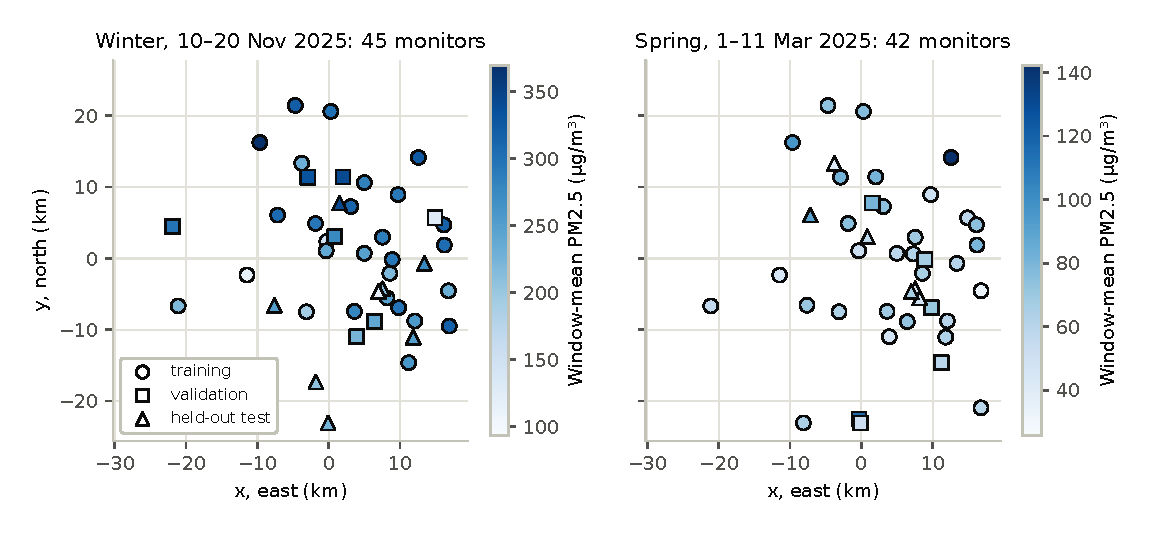
\includegraphics[width=\linewidth]{real_station_map}
\caption{Regulatory monitors used in each window, coloured by window-mean \PMtwo{} and marked by role in
the seed-42 split (OBSERVED). Axes: local tangent plane centred at $28.63^\circ$N, $77.15^\circ$E.}
\label{fig:map}
\end{figure}

\begin{figure}[htbp]
\centering
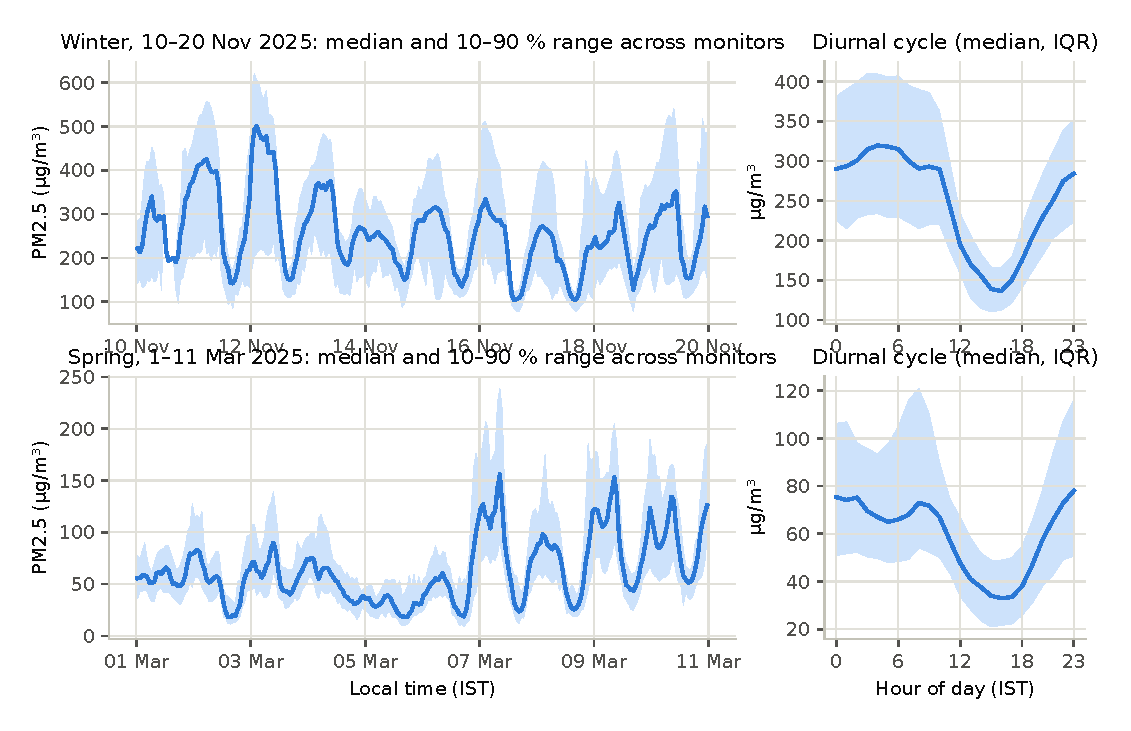
\includegraphics[width=\linewidth]{real_pm_series}
\caption{Observed hourly \PMtwo: median and 10--90\,\% range across monitors (left) and the diurnal cycle
(right). The night-time maximum and afternoon minimum mirror the diurnal cycle of the boundary layer.}
\label{fig:series}
\end{figure}

%=====================================================================
\section{Assumptions}
\label{sec:assumptions}
%=====================================================================
\begin{enumerate}
\item[A1] \textbf{Well-mixed layer.} \PMtwo{} is vertically uniform within a mixing layer of depth $H(t)$, so
the concentration measured at the surface represents the layer average. This reduces the problem from 3D to 2D.
\item[A2] \textbf{Uniform, time-varying wind.} The transporting wind $(u(t),v(t))$ is spatially uniform over the
domain and equal to the ERA5 10~m wind at the domain centre. ERA5's $\approx\SI{25}{km}$ grid cannot resolve
intra-urban variations, so we do not pretend to model them.
\item[A3] \textbf{K-theory closure.} Turbulent horizontal fluxes are $-D\nabla C$ with a constant, isotropic eddy
diffusivity $D\in[10,2000]~\si{\metre\squared\per\second}$.
\item[A4] \textbf{Linear removal.} Dry deposition and other first-order losses act at a constant rate
$\lambda=\SI{5e-6}{\per\second}$ (an $e$-folding time of 2.3 days, the order of magnitude of a deposition
velocity of $\sim\SI{0.1}{cm/s}$ over a \SI{200}{m} layer); secondary aerosol chemistry is not modelled.
\item[A5] \textbf{Separable emissions.} Emissions are a non-negative spatial flux $q(x,y)$ modulated by a 24-hour
profile $g(\tau)$ with mean one, injected into the mixing layer: $S=q\,g/\max(H,H_{\min})$, with
$H_{\min}=\SI{50}{m}$ to avoid the singularity at the very small ERA5 night-time values ($\approx$\SI{10}{m}).
\item[A6] \textbf{Boundaries.} Inflow concentrations (regional background) are unknown; we impose only a weak
zero-normal-gradient condition on outflow faces.
\item[A7] \textbf{No entrainment term.} Dilution of the layer when it deepens in the morning, and the exchange with
the residual layer, are not represented explicitly.
\end{enumerate}

%=====================================================================
\section{Mathematical formulation}
\label{sec:model}
%=====================================================================
\subsection{Governing equation}
Conservation of tracer mass in a control volume of the mixing layer, with the fluxes of A2--A3, the sink of
A4 and the source of A5, gives
\begin{equation}
\pd{C}{t} + u(t)\pd{C}{x} + v(t)\pd{C}{y} = D\left(\pd{^2C}{x^2}+\pd{^2C}{y^2}\right) - \lambda C
+ \frac{q(x,y)\,g(\tau(t))}{\max\{H(t),H_{\min}\}},
\label{eq:adr}
\end{equation}
on $\Omega\times(0,T]$, $\Omega=[x_{\min},x_{\max}]\times[y_{\min},y_{\max}]$ (\SI{49.8}{km} by \SI{53.4}{km}),
where $\tau(t)$ is the local hour. Units: $C$ in µg\,m$^{-3}$, $q$ in µg\,m$^{-2}$\,s$^{-1}$, so every term is in
µg\,m$^{-3}$\,s$^{-1}$. For the PINN the initial condition is not prescribed: $C(\cdot,0)$ is known only at
stations and enters through the data loss. On outflow faces ($\bm u\cdot\bm n>0$) we impose
$\nabla C\cdot\bm n=0$; for the synthetic truth inflow faces additionally carry the Dirichlet value
$C=C_{\mathrm{in}}$.

\subsection{Non-dimensionalisation and dimensionless groups}
With $x' = (x-x_c)/L$, $y'=(y-y_c)/L$, $t'=2t/T-1$ and $C'=C/C_{\mathrm{ref}}$, where $L=\SI{26.7}{km}$ is the
half-width, $T$ the window length and $C_{\mathrm{ref}}$ the mean training concentration, equation~\eqref{eq:adr}
becomes
\begin{equation}
\pd{C'}{t'} + U\pd{C'}{x'} + V\pd{C'}{y'} = K\nabla'^2C' - \Lambda C' + S',\qquad
U=\frac{uT}{2L},\; K=\frac{DT}{2L^2},\; \Lambda=\frac{\lambda T}{2},\; S'=\frac{S\,T}{2C_{\mathrm{ref}}}.
\label{eq:nondim}
\end{equation}
The physically meaningful groups are the P\'eclet and Damk\"ohler numbers over the domain size
$\ell\approx\SI{50}{km}$ and a typical wind $\bar u\approx\SI{1.5}{m/s}$:
\begin{equation}
\mathrm{Pe}=\frac{\bar u\,\ell}{D}\approx 75\text{--}750,\qquad
\mathrm{Da}=\frac{\lambda\,\ell}{\bar u}\approx 0.17,\qquad
t_{\mathrm{adv}}=\frac{\ell}{\bar u}\approx \SI{9}{h}.
\end{equation}
Transport is advection-dominated ($\mathrm{Pe}\gg1$), removal is weak over one transit
($\mathrm{Da}\ll1$), and air crosses the city in hours, so \emph{hourly} data can in principle see transport
between stations. For the PINN on 80-hour windows, $U\approx 5.4\,u/(\si{m/s})$, $K\approx 0.06$ and
$\Lambda\approx0.72$: all coefficients are $O(10^{-2})$--$O(10)$, which keeps the residual well scaled.

\subsection{PDE residual}
For a candidate field $\hat C'$ the residual
\begin{equation}
r = \pd{\hat C'}{t'} + U\pd{\hat C'}{x'} + V\pd{\hat C'}{y'} - K\nabla'^2\hat C' + \Lambda\hat C' - S'
\label{eq:residual}
\end{equation}
vanishes identically for an exact solution. All derivatives are computed exactly by automatic
differentiation \citep{baydin2018}.

%=====================================================================
\section{Mathematical analysis}
\label{sec:analysis}
%=====================================================================
\subsection{Stability of the continuous problem}
\begin{proposition}[Fourier stability]
For constant coefficients, the homogeneous part of \eqref{eq:adr} on $\mathbb R^2$ damps every Fourier mode.
\end{proposition}
\begin{proof}
Substituting $C=\hat c\,e^{i\bm k\cdot\bm x+\sigma t}$ gives
$\sigma = -i\,\bm u\cdot\bm k - D|\bm k|^2 - \lambda$, so $\operatorname{Re}\sigma=-(D|\bm k|^2+\lambda)<0$ for
all $\bm k$ when $D\ge0$ and $\lambda>0$. Advection only rotates the phase; diffusion damps short waves
fastest and removal damps all modes at rate $\lambda$.
\end{proof}
Consequently perturbations of the initial state are forgotten on the time scale $1/\lambda\approx\SI{56}{h}$ (or
faster, by outflow through the boundary on the scale $t_{\mathrm{adv}}$), which justifies spinning the synthetic
truth up for 24~h and not prescribing an initial field for the PINN.

\subsection{Equilibrium}
For spatially uniform, constant source $S_0$ the spatially uniform solution obeys $\dot C=S_0-\lambda C$, so
\begin{equation}
C(t)=\frac{S_0}{\lambda}+\Bigl(C_0-\frac{S_0}{\lambda}\Bigr)e^{-\lambda t}\;\longrightarrow\;C^*=\frac{S_0}{\lambda},
\end{equation}
a globally asymptotically stable equilibrium. With the diurnal factor $g(\tau)/H(t)$ the forcing is periodic and
the solution converges instead to a periodic orbit; the large day--night ratio of $H$ (up to $\sim40$ in our
windows, Figure~\ref{fig:forcing}) produces the night-time maxima seen in Figure~\ref{fig:series}. Both the decay
and the approach to $C^*$ are unit tests of our solver.

\subsection{Mass balance and positivity}
Integrating \eqref{eq:adr} over $\Omega$ gives
\begin{equation}
\frac{d}{dt}\int_\Omega C\,dA = \int_\Omega S\,dA - \lambda\int_\Omega C\,dA - \oint_{\partial\Omega}\bigl(\bm uC - D\nabla C\bigr)\cdot\bm n\,ds,
\end{equation}
so in the absence of removal, sources and boundary flux the total mass is conserved (tested to $10^{-3}$ for
the solver). By the parabolic maximum principle, $C_0\ge0$, $S\ge0$ and non-negative inflow values imply
$C\ge0$; the PINN enforces $C\ge0$ and $q\ge0$ by construction through a softplus output.

\subsection{Identifiability}
Two structural issues determine which parameters the data can constrain.
\begin{enumerate}
\item \textbf{The source can absorb the residual.} If $S$ were an unrestricted function of $(x,y,t)$, any field
$\hat C$ would satisfy \eqref{eq:residual} with $S:=\partial_t\hat C+\bm u\cdot\nabla\hat C-D\nabla^2\hat C+\lambda\hat C$,
and the physics loss would carry no information. We therefore restrict $S$ to the separable form A5
($q$: a two-layer network of 32 units with a smoothness penalty; $g$: 24 values), so the time dependence of the
source is fixed up to 24 numbers and the remaining space--time structure must be explained by transport.
\item \textbf{The diffusivity is weakly identifiable.} With $\mathrm{Pe}=O(10^2$--$10^3)$ diffusion contributes a
small fraction of the transport; changes in $D$ barely alter concentrations at the stations
(Section~\ref{sec:sens}). We therefore expect $D$ to be poorly determined, and test this directly.
\end{enumerate}

\subsection{Forward sensitivity}
\label{sec:sens}
We re-ran the reference solver of Section~\ref{sec:numerics} with one parameter varied at a time and sampled
the result at the 45 monitor locations (Figure~\ref{fig:sens}). Over the ranges shown the elasticity
$\partial\ln\bar C/\partial\ln p$ of the station-mean concentration is $-0.15$ for $\lambda$, $-0.03$ for $D$ and
$-0.35$ for $H_{\min}$. The near-zero sensitivity to $D$ is the quantitative form of the identifiability
argument; the mixing-height floor, a modelling choice, matters more than either physical rate.

\begin{figure}[htbp]
\centering
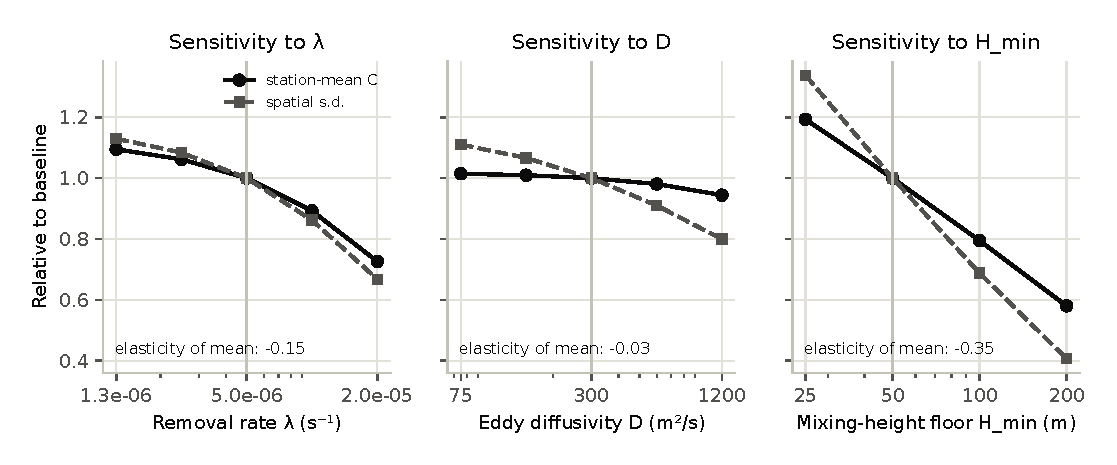
\includegraphics[width=\linewidth]{twin_forward_sensitivity}
\caption{Forward-model sensitivity of station concentrations to $\lambda$, $D$ and $H_{\min}$ (one at a time,
reference solver, 3-day winter forcing). Values relative to the baseline run.}
\label{fig:sens}
\end{figure}

%=====================================================================
\section{Numerical methodology}
\label{sec:numerics}
%=====================================================================
\subsection{Reference finite-difference solver}
For the synthetic twin and for verification we solve \eqref{eq:adr} by the method of lines on a
cell-centred grid ($\Delta x=\Delta y=\SI{1}{km}$, $51\times54$ cells) \citep{hundsdorfer2003}: third-order
upwind-biased differences for advection (for $u>0$,
$\partial_xC_i\approx(2C_{i+1}+3C_i-6C_{i-1}+C_{i-2})/6\Delta x$), second-order central differences for diffusion,
and the strong-stability-preserving third-order Runge--Kutta method in time \citep{gottlieb1998}. Two ghost cells
carry Dirichlet values on inflow faces and zero-gradient extrapolation on outflow faces.

\paragraph{Stability (von Neumann).} For the central diffusion operator the semi-discrete symbol is
$-\tfrac{4D}{\Delta x^2}\sin^2\tfrac{\theta_x}{2}-\tfrac{4D}{\Delta y^2}\sin^2\tfrac{\theta_y}{2}$, whose most negative
value is $-4D(\Delta x^{-2}+\Delta y^{-2})$. SSP-RK3 is stable on the negative real axis up to $|z|\approx2.51$, so
explicit stability requires $D\Delta t(\Delta x^{-2}+\Delta y^{-2})\lesssim0.63$; we use $0.25$. For advection we
limit the Courant number $\Delta t(|u|/\Delta x+|v|/\Delta y)\le0.5$, inside the stability region of the
upwind-biased/RK3 combination. The time step is the smaller of the two limits.

\paragraph{Verification.} The solver reproduces pure exponential decay and the approach to $C^*=S_0/\lambda$ to a
relative error of $10^{-5}$, conserves mass to $10^{-3}$, and converges to the exact advected--diffusing Gaussian puff
\begin{equation}
C(\bm x,t)=\frac{M}{4\pi Dt}\exp\!\Bigl(-\frac{|\bm x-\bm x_0-\bm ut|^2}{4Dt}-\lambda t\Bigr)
\label{eq:puff}
\end{equation}
with relative $L^2$ errors $1.4\times10^{-2}$, $1.1\times10^{-3}$ and $1.9\times10^{-4}$ on \SIlist{750;375;188}{m} grids
(observed orders 3.7 and 2.6, consistent with third-order advection combined with second-order diffusion).

\subsection{PINN architecture}
\begin{figure}[htbp]
\centering
\resizebox{\linewidth}{!}{%
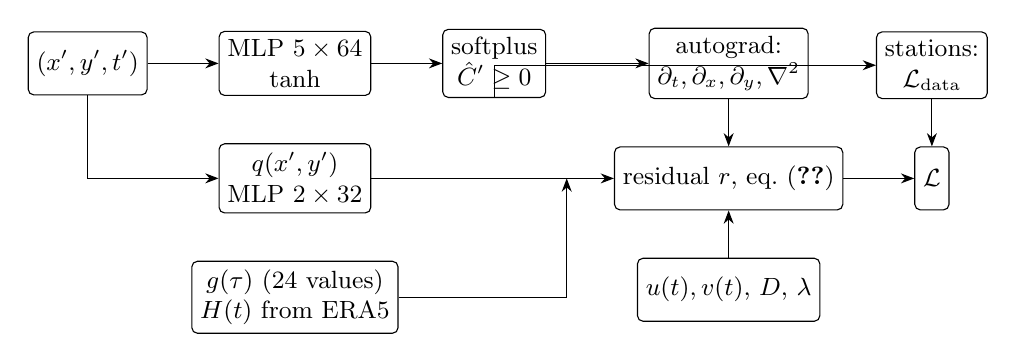
\begin{tikzpicture}[>=Stealth, node distance=6mm and 9mm,
  box/.style={draw, rounded corners=2pt, align=center, font=\small, minimum height=8mm, inner sep=3pt},
  op/.style={draw, circle, font=\small, inner sep=1pt}]
\node[box] (in) {$(x',y',t')$};
\node[box, right=of in] (mlp) {MLP $5\times64$\\ $\tanh$};
\node[box, right=of mlp] (out) {softplus\\ $\hat C'\ge0$};
\node[box, below=of mlp] (q) {$q(x',y')$\\ MLP $2\times32$};
\node[box, below=of q] (gH) {$g(\tau)$ (24 values)\\ $H(t)$ from ERA5};
\node[box, right=of out, xshift=4mm] (ad) {autograd:\\ $\partial_t,\partial_x,\partial_y,\nabla^2$};
\node[box, below=of ad] (res) {residual $r$, eq.~\eqref{eq:residual}};
\node[box, right=of res] (loss) {$\mathcal L$};
\node[box, above=of loss] (data) {stations:\\ $\mathcal L_{\mathrm{data}}$};
\node[box, below=of res] (wind) {$u(t),v(t)$, $D$, $\lambda$};
\draw[->] (in) -- (mlp); \draw[->] (mlp) -- (out); \draw[->] (out) -- (ad); \draw[->] (ad) -- (res);
\draw[->] (in) |- (q); \draw[->] (q) -| ([xshift=-6mm]res.west) -- (res.west);
\draw[->] (gH) -| ([xshift=-6mm]res.west);
\draw[->] (wind) -- (res); \draw[->] (res) -- (loss); \draw[->] (data) -- (loss);
\draw[->] (out) |- (data);
\end{tikzpicture}}
\caption{PINN architecture. The concentration network and the source model are trained jointly with the
bounded diffusivity $D$; wind and mixing height are fixed inputs to the residual.}
\label{fig:arch}
\end{figure}

The concentration network (Figure~\ref{fig:arch}) maps dimensionless $(x',y',t')\in[-1,1]^3$ to
\[
\hat C'=\operatorname{softplus}\bigl(\mathrm{MLP}(x',y',t')\bigr),
\]
with five hidden layers of 64 units, $\tanh$ activations and Glorot initialisation \citep{glorot2010}. The activation must be smooth: with ReLU the second derivatives
in the diffusion term would vanish almost everywhere. Meteorology is \emph{not} an input, so that
$\partial\hat C/\partial t$ is the true partial derivative of the field; it enters only through the coefficients of
\eqref{eq:nondim}. The diffusivity is $D=D_{\min}+(D_{\max}-D_{\min})\,\sigma(\theta_D)$ with $\sigma$ the logistic
function, initialised at \SI{300}{m^2/s}.

\subsection{Loss function}
With $N_d$ training observations, $N_c$ collocation points and $N_b$ boundary points,
\begin{align}
\mathcal L &= w_d\mathcal L_{\mathrm{data}} + w_p\mathcal L_{\mathrm{phys}} + w_b\mathcal L_{\mathrm{bc}}
+ w_i\mathcal L_{\mathrm{ic}} + w_s\mathcal L_{\mathrm{src}},\\
\mathcal L_{\mathrm{data}} &= \frac1{N_d}\sum_{j}\bigl(\hat C'(\bm z_j)-C'_j\bigr)^2,\qquad
\mathcal L_{\mathrm{phys}} = \frac1{N_c}\sum_{k} r(\bm z_k)^2,\\
\mathcal L_{\mathrm{bc}} &= \frac1{N_b}\sum_{m}\mathbb 1[\bm u\cdot\bm n_m>0]\,\bigl(\nabla\hat C'\cdot\bm n_m\bigr)^2,\qquad
\mathcal L_{\mathrm{src}} = \overline{|\nabla q|^2} + \tfrac1{24}\textstyle\sum_h (g_{h+1}-2g_h+g_{h-1})^2 .
\end{align}
$\mathcal L_{\mathrm{ic}}$ (misfit to a known initial field) is used only for testing: on real data the initial
field is known only at stations and is already part of $\mathcal L_{\mathrm{data}}$. We use $w_d=1$, $w_b=0.1$,
$w_s=10^{-3}$, $w_i=0$, and select $w_p$ as described in Section~\ref{sec:twin}. The \emph{data-only network} is
the identical model and optimiser with $w_p=w_b=w_s=0$; only its concentration network is trained.

\paragraph{Training.} Adam \citep{kingma2015} for 6000 iterations with the learning rate decaying exponentially from
$10^{-3}$ to $10^{-4}$; 4096 collocation points (Latin hypercube \citep{mckay1979}) and 512 boundary points,
resampled every 250 iterations. Validation stations are evaluated every 100 iterations and the weights with the
lowest validation error are kept; validation stations never contribute gradients. Implementation in PyTorch
\citep{paszke2019}. We also implemented gradient-norm balancing of $w_p$ \citep{wang2021}; started from $w_p=1$ it
adapted too slowly and was not competitive, so we report fixed weights.

\paragraph{Time-domain decomposition.} The twin windows are 73~h long. Real windows are 240~h; the advective
coefficient $U$ grows with $T$ and a single network must represent ten diurnal cycles, both known causes of PINN
failure \citep{krishnapriyan2021}. We therefore split each real window into three consecutive 80-hour chunks and
train one data-only network and one PINN per chunk.

\subsection{Evaluation protocol}
Stations, not observations, are split into training (70\,\%), validation (15\,\%) and test (15\,\%) sets. Stations
closer than \SI{1}{km} (co-located instruments, e.g.\ two at Pusa) are grouped so that a test station never has a
near-duplicate in training; leakage is asserted in code. All models use the same split. We repeat with three or four
splits (seeds) and report mean $\pm$ standard deviation of MAE, RMSE, $R^2$ and bias at the test stations. Baselines:
the hourly mean of the training stations (a spatially uniform field), inverse-distance weighting with power 2
\citep{shepard1968}, and a random forest \citep{breiman2001} on $(x,y,t)$, hour of day and ERA5 $u,v,H$.

%=====================================================================
\section{Numerical simulations: the synthetic twin}
\label{sec:twin}
%=====================================================================
\paragraph{Design.} The truth is the solution of \eqref{eq:adr} by the reference solver with $D=\SI{300}{m^2/s}$,
$\lambda=\SI{5e-6}{s^{-1}}$, inflow $C_{\mathrm{in}}=\SI{60}{\micro\gram\per\metre\cubed}$, a background flux of
\SI{0.4}{\micro\gram\per\metre\squared\per\second} plus three Gaussian hotspots (illustrative, not an inventory), and a
traffic-like diurnal profile, driven by the \emph{real} ERA5 forcing of 12--15 November 2024 (Figure~\ref{fig:forcing})
after a 24-hour spin-up. It is sampled hourly at the 45 real monitor locations with 5\,\% multiplicative noise
(Figure~\ref{fig:twinmap}). The twin is \emph{model-correct}: the PINN's structural form matches the truth, so it
measures what the method can achieve when its assumptions hold, and lets us score the whole field, not just stations.

\begin{figure}[htbp]
\centering
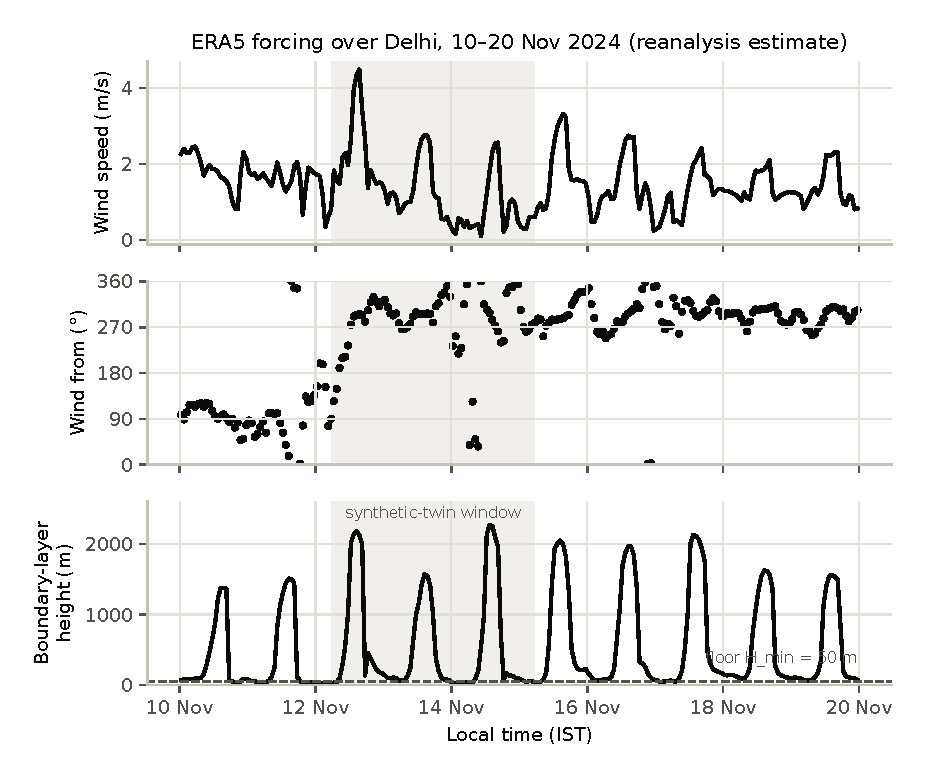
\includegraphics[width=0.85\linewidth]{era5_forcing}
\caption{ERA5 forcing used for the synthetic twin (estimated quantities). Grey band: the 3-day twin window.}
\label{fig:forcing}
\end{figure}

\begin{figure}[htbp]
\centering
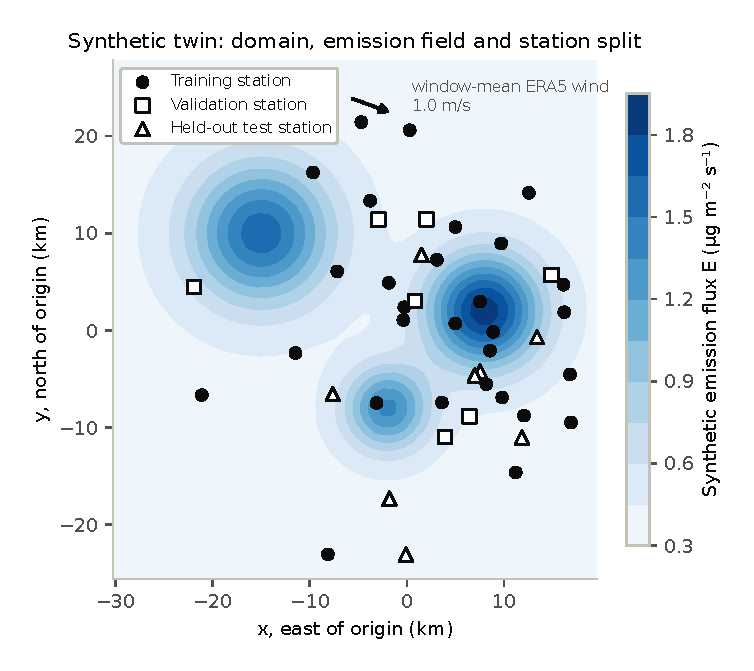
\includegraphics[width=0.62\linewidth]{twin_study_area}
\caption{Synthetic emission field and the station split (seed 42) at the real monitor locations.}
\label{fig:twinmap}
\end{figure}

\paragraph{Choice of the physics weight.} Figure~\ref{fig:wp} shows the effect of $w_p$. At $w_p=1$ the physics term
dominates the gradient (its initial value is $\approx12$ against $\approx0.55$ for the data term) and the optimiser
under-fits the data, a manifestation of the imbalance described by \citet{wang2021}; accuracy improves steadily as
$w_p$ decreases to $0.003$--$0.01$. We fixed $w_p=0.01$ for all subsequent experiments, including the real data,
\emph{before} running them.

\begin{figure}[htbp]
\centering
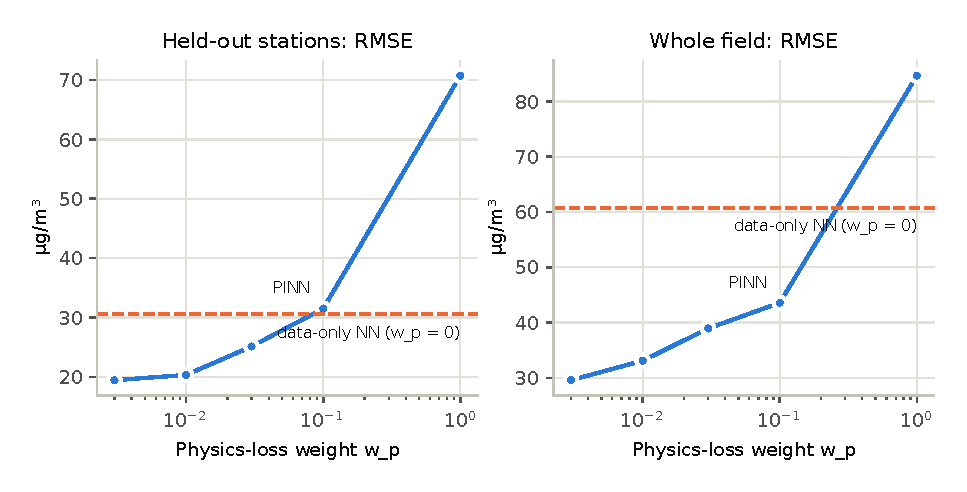
\includegraphics[width=0.85\linewidth]{twin_wp_sweep}
\caption{Synthetic twin: held-out-station and whole-field RMSE against $w_p$ (seed 42).}
\label{fig:wp}
\end{figure}

%=====================================================================
\section{Results and interpretation}
\label{sec:results}
%=====================================================================
\subsection{Synthetic twin}
\begin{table}[htbp]
\centering\small
\caption{Synthetic twin, held-out stations (mean $\pm$ s.d.\ over 4 splits; µg/m$^3$). Field RMSE is against the
known truth on the 1~km grid every 3~h.}
\label{tab:twin}
\begin{tabular}{@{}lccc@{}}
\toprule
Model & RMSE & MAE & Field RMSE \\
\midrule
IDW & $43.8\pm9.5$ & $28.8\pm6.4$ & --- \\
Random forest & $43.8\pm5.6$ & $27.0\pm3.0$ & --- \\
Data-only NN & $29.9\pm9.9$ & $18.9\pm3.9$ & $54.5\pm9.6$ \\
\textbf{PINN} ($w_p=0.01$) & $\mathbf{22.1\pm3.1}$ & $\mathbf{15.1\pm1.6}$ & $\mathbf{31.3\pm2.3}$ \\
\bottomrule
\end{tabular}
\end{table}

Table~\ref{tab:twin} and Figure~\ref{fig:twincomp} summarise the twin. The PINN has the lowest error and, notably,
the smallest spread across splits. It beats the data-only network at the held-out stations in three of four splits
and on the whole field in all four, by 43\,\% on average: the improvement is largest away from stations, where the
data alone say nothing and the PDE propagates information along the wind (Figure~\ref{fig:fields}; the PINN has the
lower field error in 72 of 73 hours for seed 42). The same experiment on an earlier, randomly placed 36-station
layout gave the same ordering (RMSE $24.9\pm6.8$ versus $31.2\pm8.7$; field $31.5$ versus $49.3$), so the result does not
depend on the station geometry. Figure~\ref{fig:train} shows why early stopping matters for the data-only network:
its validation error rises after $\approx2000$ iterations while the PINN's keeps falling.

\begin{figure}[htbp]
\centering
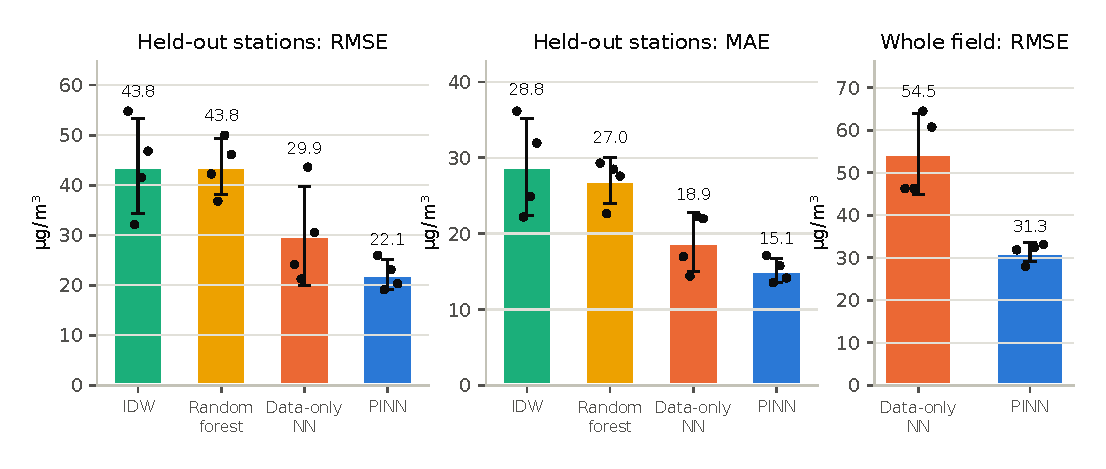
\includegraphics[width=\linewidth]{twin_comparison}
\caption{Synthetic twin: model comparison over four station splits (dots: individual splits).}
\label{fig:twincomp}
\end{figure}

\begin{figure}[htbp]
\centering
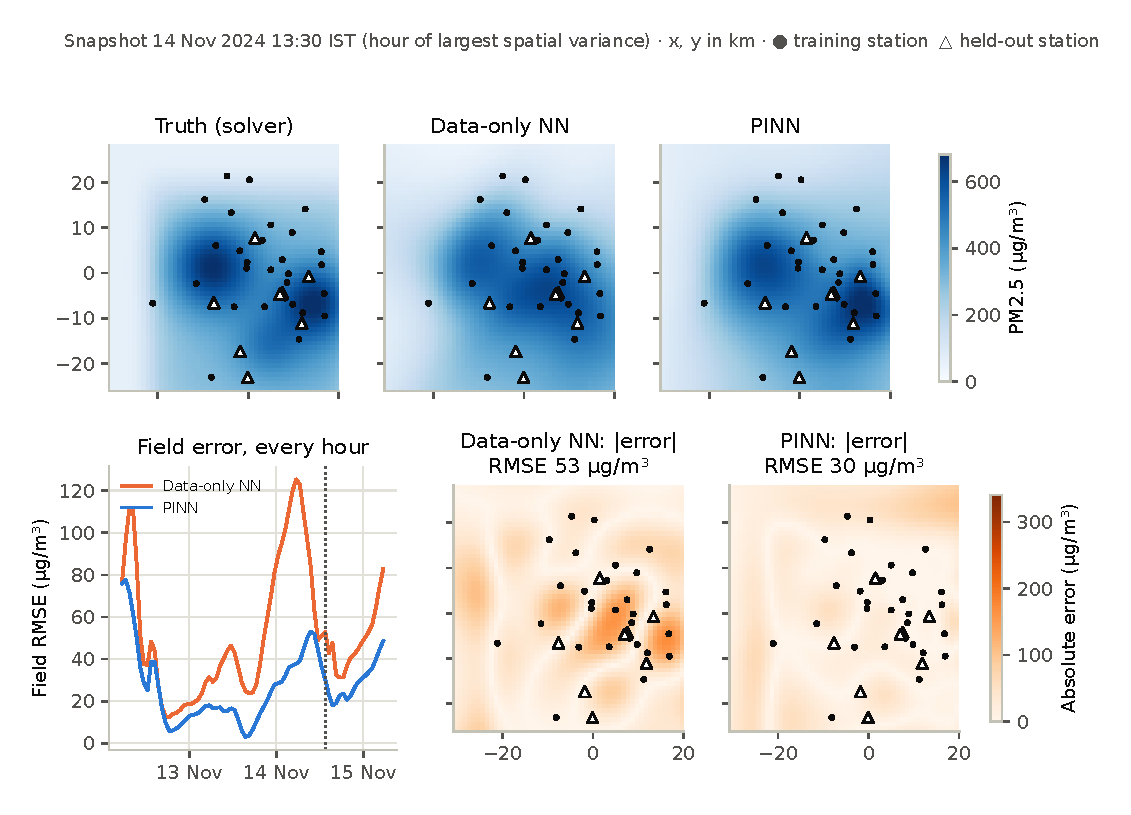
\includegraphics[width=\linewidth]{twin_fields}
\caption{Synthetic twin: truth and reconstructions at the hour of largest spatial variance (chosen by rule, seed 42),
absolute errors, and field RMSE at every hour. Every panel is a model evaluated on the grid.}
\label{fig:fields}
\end{figure}

\begin{figure}[htbp]
\centering
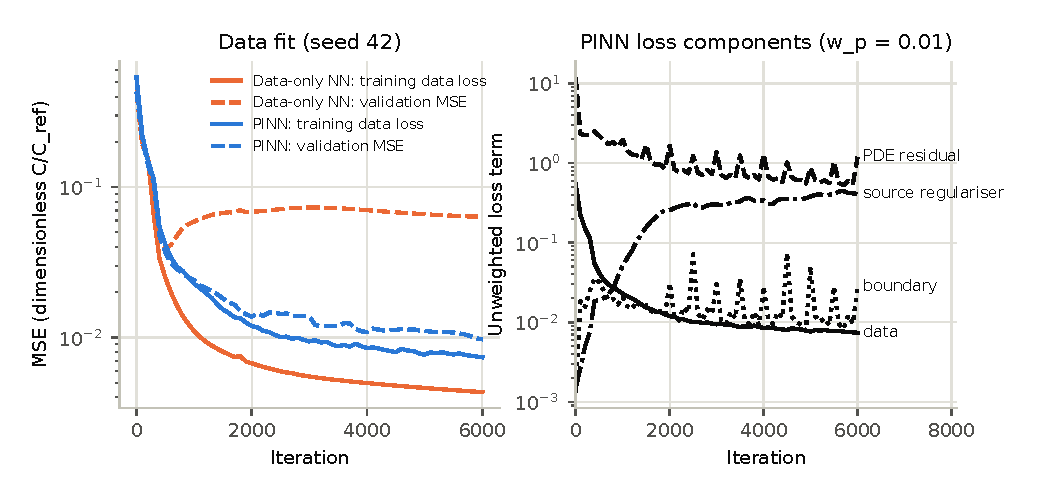
\includegraphics[width=\linewidth]{twin_training}
\caption{Synthetic twin training history (seed 42). Left: data and validation losses. Right: unweighted PINN loss terms.}
\label{fig:train}
\end{figure}

\paragraph{Physical consistency.} The PINN's fields satisfy the PDE far better than the data-only network's: its median
residual is $0.35$ against $1.35$ even after we freeze the data-only field and fit an emission model and $D$ to it
(Figure~\ref{fig:twinres}). Fitting the stations is therefore not sufficient to produce a transport-consistent field.

\begin{figure}[htbp]
\centering
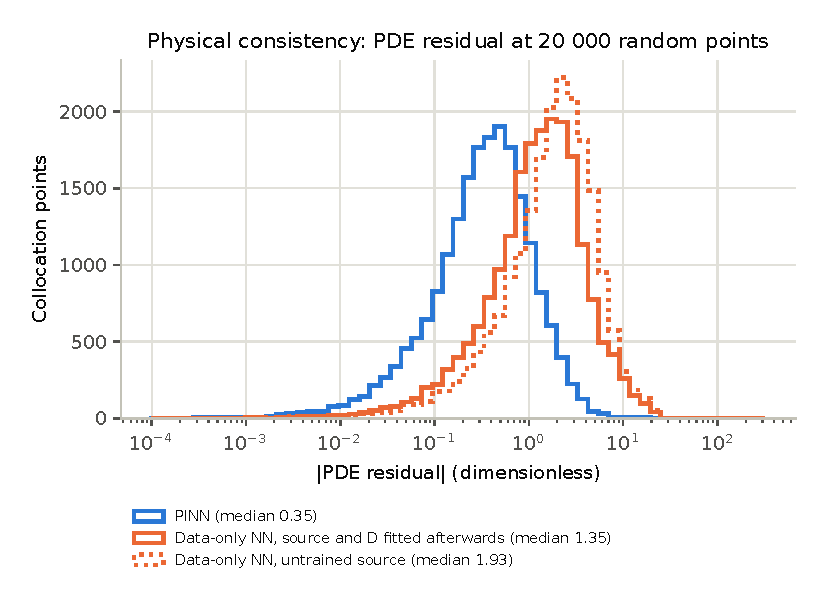
\includegraphics[width=0.8\linewidth]{twin_residual}
\caption{Synthetic twin: absolute PDE residual at 20\,000 random points (seed 42).}
\label{fig:twinres}
\end{figure}

\paragraph{Parameter recovery.} Figure~\ref{fig:ident} confirms the identifiability analysis. Although $D$ was
initialised at its true value of \SI{300}{m^2/s}, every split drives it to 58--60~m$^2$/s: the data are consistent
with a broad range of diffusivities and the optimiser trades diffusion for other degrees of freedom. The diurnal
profile, by contrast, is recovered well (both peaks and the night-time minimum), with the evening peak about an hour late.

\begin{figure}[htbp]
\centering
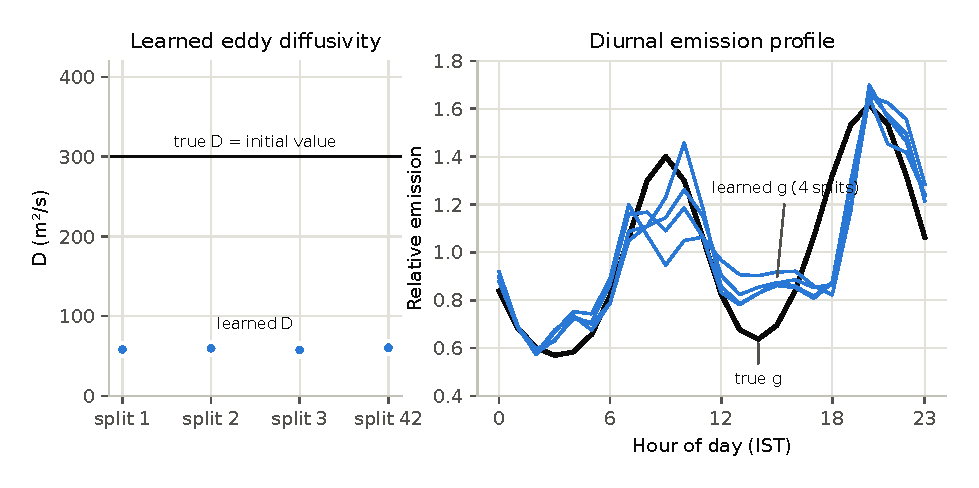
\includegraphics[width=0.9\linewidth]{twin_identifiability}
\caption{Synthetic twin: learned $D$ against the truth, and learned versus true diurnal profile.}
\label{fig:ident}
\end{figure}

\subsection{Observed data}
\begin{table}[htbp]
\centering\small
\caption{Observed \PMtwo, held-out monitors: RMSE (µg/m$^3$), mean $\pm$ s.d.\ over 3 splits; 6--8 test monitors and
1\,372--1\,726 test hours per run. $w_p=0.01$ fixed in advance.}
\label{tab:real}
\begin{tabular}{@{}lcc@{}}
\toprule
Model & Winter (mean 258) & Spring (mean 67) \\
\midrule
Training-station mean & $84.8\pm21.2$ & $\mathbf{29.7\pm4.6}$ \\
IDW & $84.4\pm19.2$ & $33.2\pm3.8$ \\
Random forest & $94.2\pm20.4$ & $36.8\pm4.1$ \\
Data-only NN & $111.4\pm62.5$ & $41.4\pm2.8$ \\
PINN & $\mathbf{83.3\pm24.7}$ & $33.1\pm3.7$ \\
\bottomrule
\end{tabular}
\end{table}

Table~\ref{tab:real} and Figures~\ref{fig:realcomp}--\ref{fig:realseries} give the real-data results. Three findings stand out.

\begin{enumerate}
\item \textbf{Physics regularises the network.} The PINN is better than the identical data-only network in all six
runs, and much more stable: the data-only network's winter RMSE ranges from 65 to 182~µg/m$^3$ across splits, the PINN's
from 61 to 110.
\item \textbf{The PINN's fields are more physically consistent.} Its median PDE residual is $0.61$ (winter) and
$0.50$ (spring), against $2.24$ and $4.13$ for the data-only field with a post-hoc fitted source
(Figure~\ref{fig:realres}).
\item \textbf{The PINN does not beat simple spatial baselines.} In winter, PINN, IDW and the station mean differ by less
than 2~µg/m$^3$, far less than the spread between splits; in spring the training-station mean, which has no spatial
structure at all, is best. The PINN is best in only one of the six runs.
\end{enumerate}

\begin{figure}[htbp]
\centering
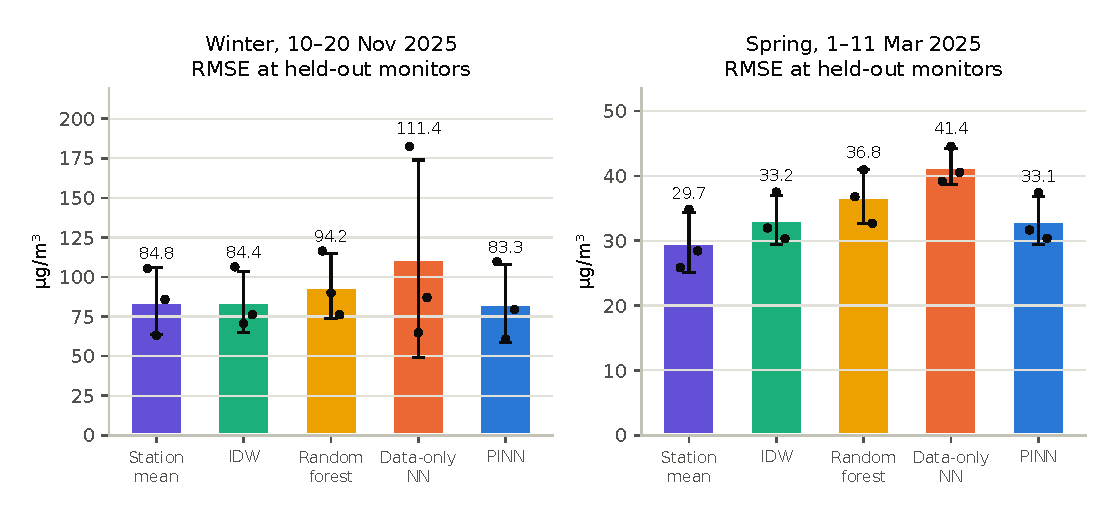
\includegraphics[width=\linewidth]{real_comparison}
\caption{Observed data: RMSE at held-out monitors over three splits (dots: individual splits).}
\label{fig:realcomp}
\end{figure}

\begin{figure}[htbp]
\centering
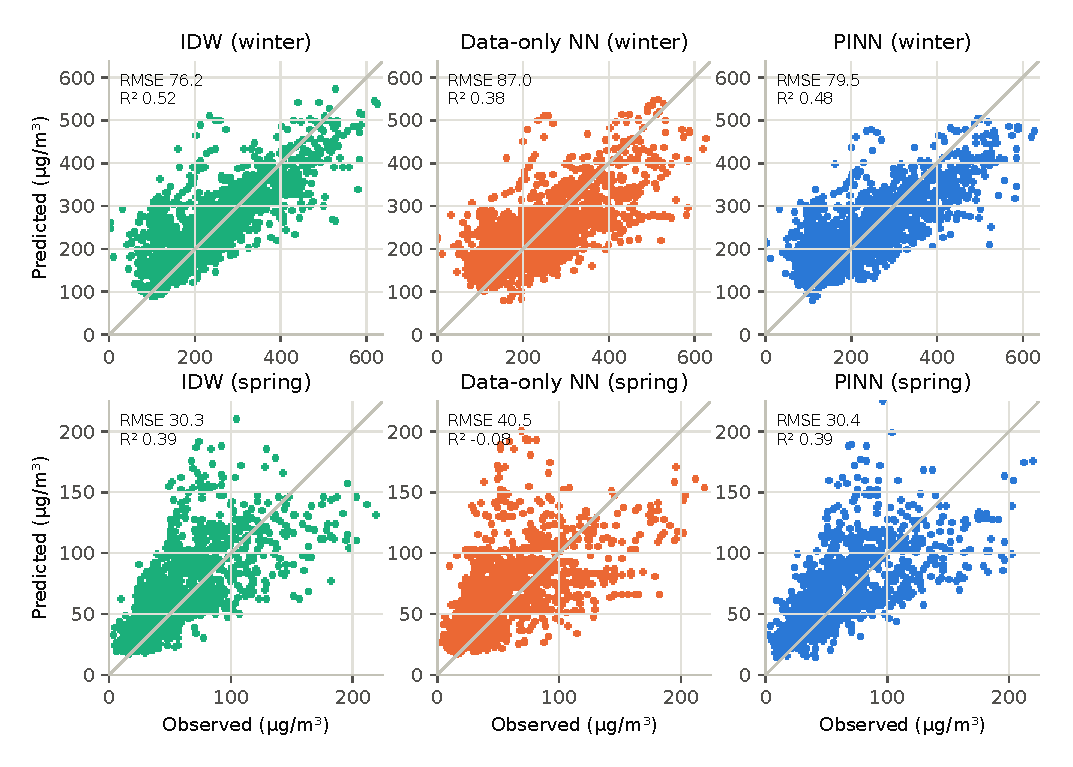
\includegraphics[width=0.9\linewidth]{real_parity}
\caption{Observed data: predicted against measured \PMtwo{} at held-out monitors (seed 42).}
\label{fig:realparity}
\end{figure}

\begin{figure}[htbp]
\centering
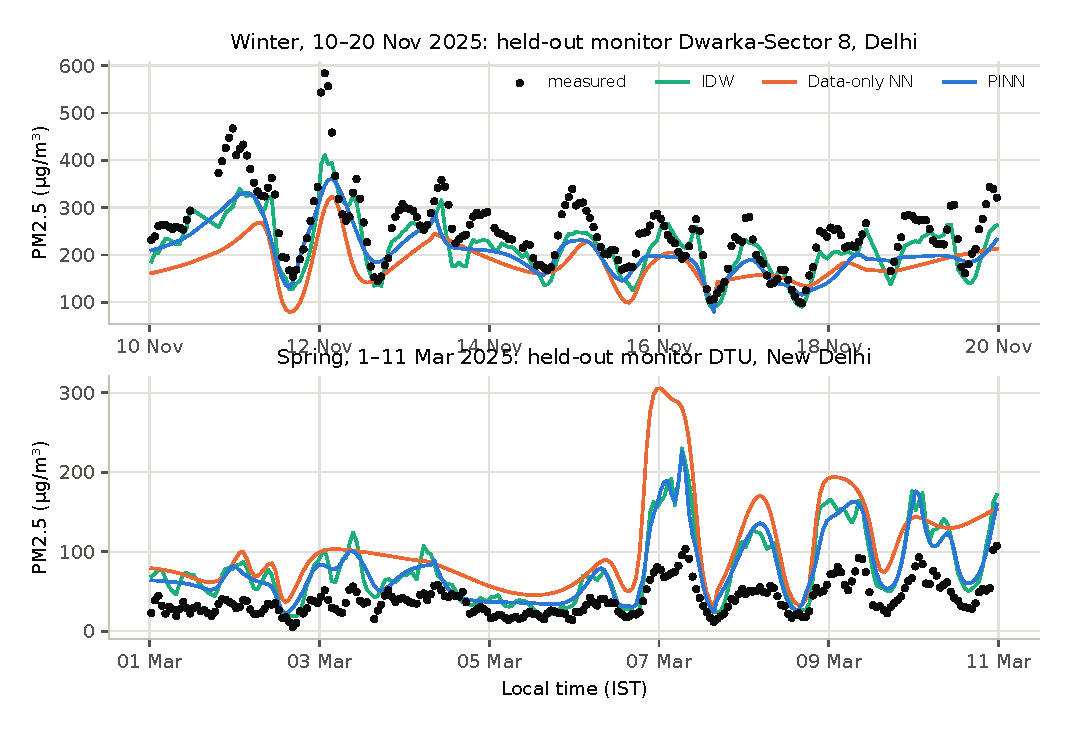
\includegraphics[width=0.95\linewidth]{real_station_series}
\caption{Observed data: one held-out monitor per window and its reconstructions (seed 42).}
\label{fig:realseries}
\end{figure}

\begin{figure}[htbp]
\centering
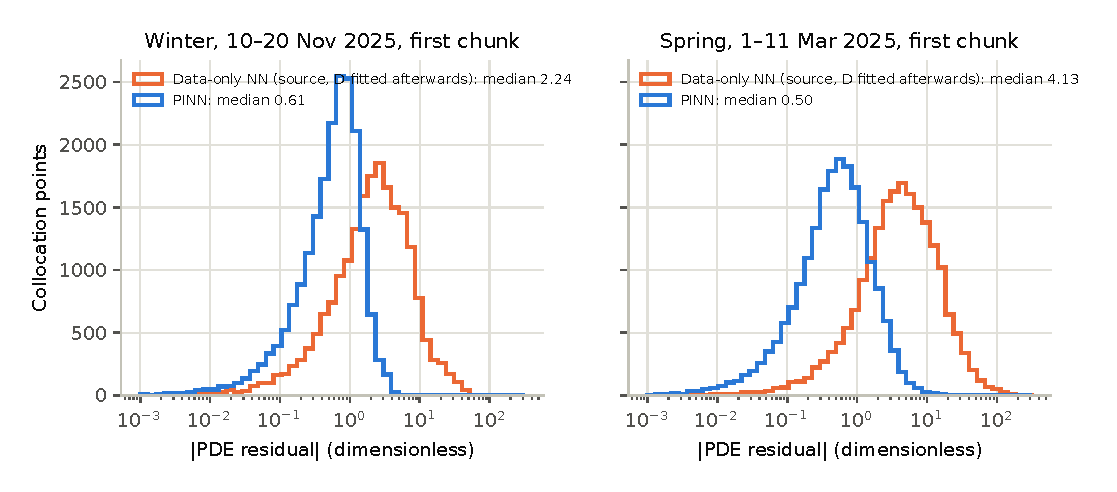
\includegraphics[width=0.95\linewidth]{real_residual}
\caption{Observed data: PDE residual in the first 80-hour chunk (seed 42).}
\label{fig:realres}
\end{figure}

\paragraph{Why the physics does not help more on real data.} The contrast with the twin isolates the cause: the
method works when the model is right, so the shortfall on real data reflects the model's mismatch with Delhi's atmosphere.
\begin{itemize}
\item \emph{A strong common signal.} The median inter-station correlation is about $0.7$. A spatially uniform estimate
already captures most of the variance at an unseen station, leaving little that transport between stations can add.
\item \emph{Uniform wind.} The monitors' own anemometers (winter only; the March 2025 archive files contain no wind data)
correlate with the ERA5 wind at $r=0.50$ and read much lower ($0.55$ versus \SI{1.38}{m/s}; Figure~\ref{fig:wind}).
Rooftop instruments in the urban canopy are expected to read low, but the moderate correlation means that the
transporting wind, and certainly its spatial variation, are uncertain.
\item \emph{Missing processes.} The model has no entrainment term (A7), no regional inflow (A6) and no secondary aerosol
formation (A4). Regional transport during the post-monsoon season enters the domain through the boundaries, which the PINN
cannot represent except through the learned source.
\item \emph{Unidentified diffusivity.} Across the 18 real-data chunks the learned $D$ ranges from 37 to 266~m$^2$/s with
no consistent value, as on the twin.
\end{itemize}
The sweep in Figure~\ref{fig:realwp} shows that the conclusion does not hinge on the a-priori choice $w_p=0.01$: over
$w_p\in\{0.003,0.01,0.03\}$ the PINN's winter RMSE stays between 78.5 and 81.0 and its spring RMSE between 30.4 and 32.8,
always better than the data-only network and never clearly better than IDW.

\begin{figure}[htbp]
\centering
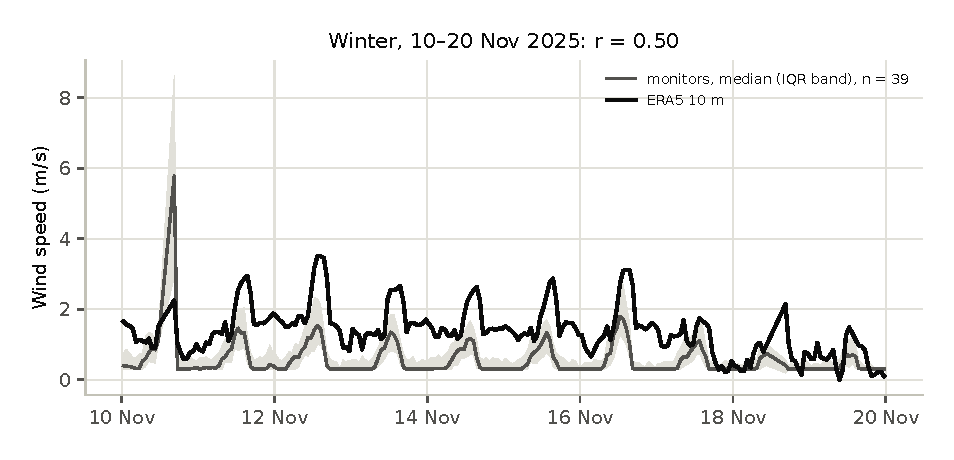
\includegraphics[width=0.8\linewidth]{real_wind_check}
\caption{Monitor anemometers (median and IQR, 39 stations) against the ERA5 wind used in the PDE, winter window.}
\label{fig:wind}
\end{figure}

\begin{figure}[htbp]
\centering
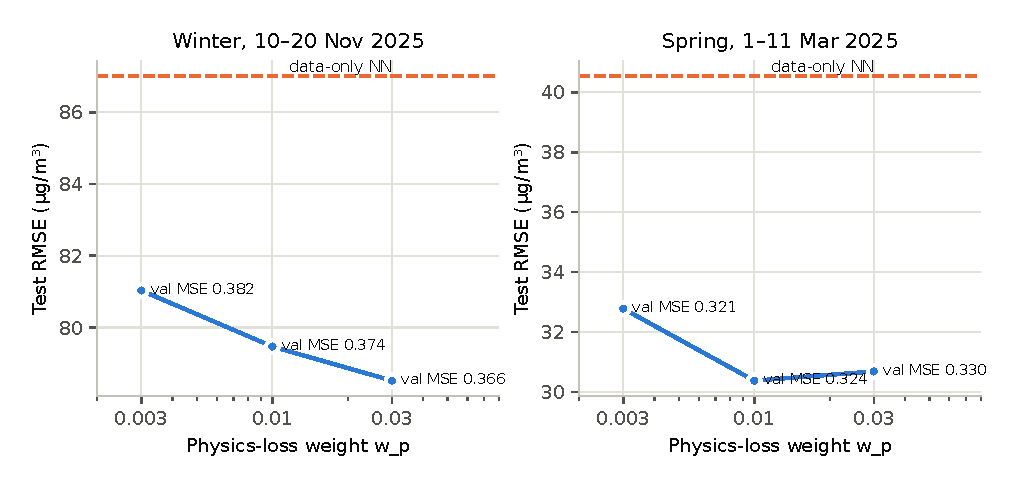
\includegraphics[width=0.85\linewidth]{real_wp_sweep}
\caption{Observed data: PINN test RMSE against $w_p$ (seed 42); labels give the validation MSE.}
\label{fig:realwp}
\end{figure}

%=====================================================================
\FloatBarrier
\section{Limitations}
%=====================================================================
\begin{itemize}
\item \textbf{Model structure.} Two-dimensional, well-mixed, uniform-wind transport with constant $D$ and $\lambda$ and no
chemistry or entrainment (A1--A7). The real-data results indicate that these simplifications, not the PINN method,
limit accuracy.
\item \textbf{Boundary conditions.} Inflow concentrations are unknown; only a weak outflow condition is imposed. A regional
background (for example from a chemical transport model, labelled as model output) would be the natural next step.
\item \textbf{Sparse data and short windows.} 30 training stations, 6--8 test stations and two ten-day windows give wide
uncertainty bands; with three splits per window, differences of a few µg/m$^3$ are not significant.
\item \textbf{Synthetic twin is optimistic.} It shares the PINN's structural form, so it is an upper bound on performance.
\item \textbf{Optimisation.} Results depend on $w_p$, iteration count and time-domain decomposition; adaptive weighting
did not help in our implementation. Repeated runs on different CPU thread counts differ in the last digit.
\item \textbf{Data provenance.} OpenAQ redistributes CPCB/DPCC data; gaps in the archive (November 2024) forced a change of
window, and timestamps of 15-minute values were aggregated by hour, which may shift averages by up to one hour.
\end{itemize}

%=====================================================================
\section{Conclusion}
%=====================================================================
We built and analysed a two-dimensional advection--diffusion--reaction model of Delhi's \PMtwo{} whose inputs are
measured, estimated from reanalysis or learned, verified its numerical and automatic-differentiation implementations
against exact solutions, and trained a PINN on it. When the model's assumptions hold (synthetic twin with real
forcing and real station locations), the physics constraint reduces the error at unseen stations by 26\,\% and the
error over the whole field by 43\,\% relative to an identical network without physics, and produces fields that are
consistent with transport. On observed data the physics still stabilises the network and enforces physical
consistency, but the simplified model does not capture enough of the real variability to beat simple interpolation.
The analysis explains the outcome: Delhi's \PMtwo{} is dominated by a spatially coherent signal, the eddy diffusivity is
not identifiable at P\'eclet numbers of $10^2$--$10^3$, and processes we omitted (regional inflow, entrainment, local wind
structure) carry much of the residual variability. A physics-informed model is only as useful as the physics it encodes;
the clearest routes to improvement are a regional boundary condition and a mixing-height entrainment term.

\paragraph{Reproducibility.} All code, tests (50, \texttt{pytest}), configuration and seeds are in the project
repository; \texttt{data/README.md} documents data download and provenance, and every figure is regenerated by
\texttt{experiments/make\_figures\_twin.py} and \texttt{experiments/make\_figures\_real.py}.

\FloatBarrier
\bibliographystyle{plainnat}
\bibliography{references}

\end{document}
